%%%%%%%%%%%%%%%%%%%%%%%%%%%%%%%%%%%%%%%%%
% Structured General Purpose Assignment
% LaTeX Template
%
% This template has been downloaded from:
% http://www.latextemplates.com
%
% Original author:
% Ted Pavlic (http://www.tedpavlic.com)
%
% Note:
% The \lipsum[#] commands throughout this template generate dummy text
% to fill the template out. These commands should all be removed when
% writing assignment content.
%
%%%%%%%%%%%%%%%%%%%%%%%%%%%%%%%%%%%%%%%%%

%----------------------------------------------------------------------------------------
%	PACKAGES AND OTHER DOCUMENT CONFIGURATIONS
%----------------------------------------------------------------------------------------

\documentclass{article}

\usepackage{multirow}
\usepackage{amssymb}
\usepackage[fleqn]{amsmath}
\usepackage{url}

\usepackage{fancyhdr} % Required for custom headers
\usepackage{lastpage} % Required to determine the last page for the footer
\usepackage{extramarks} % Required for headers and footers
\usepackage{graphicx} % Required to insert images
\usepackage{lipsum} % Used for inserting dummy 'Lorem ipsum' text into the template

% Margins
\topmargin=-0.45in
\evensidemargin=0in
\oddsidemargin=0in
\textwidth=6.5in
\textheight=9.0in
\headsep=0.25in

\linespread{1.1} % Line spacing

% Set up the header and footer
\pagestyle{fancy}
\lhead{\hmwkAuthorName} % Top left header
\chead{\hmwkClass\ : \hmwkTitle} % Top center header
\rhead{\firstxmark} % Top right header
\lfoot{\lastxmark} % Bottom left footer
\cfoot{} % Bottom center footer
\rfoot{Page\ \thepage\ of\ \pageref{LastPage}} % Bottom right footer
\renewcommand\headrulewidth{0.4pt} % Size of the header rule
\renewcommand\footrulewidth{0.4pt} % Size of the footer rule

\setlength\parindent{0pt} % Removes all indentation from paragraphs

%----------------------------------------------------------------------------------------
%	DOCUMENT STRUCTURE COMMANDS
%	Skip this unless you know what you're doing
%----------------------------------------------------------------------------------------

% Header and footer for when a page split occurs within a problem environment
\newcommand{\enterProblemHeader}[1]{
\nobreak\extramarks{#1}{#1 continued on next page\ldots}\nobreak
\nobreak\extramarks{#1 (continued)}{#1 continued on next page\ldots}\nobreak
}

% Header and footer for when a page split occurs between problem environments
\newcommand{\exitProblemHeader}[1]{
\nobreak\extramarks{#1 (continued)}{#1 continued on next page\ldots}\nobreak
\nobreak\extramarks{#1}{}\nobreak
}

\setcounter{secnumdepth}{0} % Removes default section numbers
\newcounter{homeworkProblemCounter} % Creates a counter to keep track of the number of problems

\newcommand{\homeworkProblemName}{}
\newenvironment{homeworkProblem}[1][Problem \arabic{homeworkProblemCounter}]{ % Makes a new environment called homeworkProblem which takes 1 argument (custom name) but the default is "Problem #"
\stepcounter{homeworkProblemCounter} % Increase counter for number of problems
\renewcommand{\homeworkProblemName}{#1} % Assign \homeworkProblemName the name of the problem
\section{\homeworkProblemName} % Make a section in the document with the custom problem count
\enterProblemHeader{\homeworkProblemName} % Header and footer within the environment
}{
\exitProblemHeader{\homeworkProblemName} % Header and footer after the environment
}

\newcommand{\problemAnswer}[1]{ % Defines the problem answer command with the content as the only argument
\noindent\framebox[\columnwidth][c]{\begin{minipage}{0.98\columnwidth}#1\end{minipage}} % Makes the box around the problem answer and puts the content inside
}

\newcommand{\homeworkSectionName}{}
\newenvironment{homeworkSection}[1]{ % New environment for sections within homework problems, takes 1 argument - the name of the section
\renewcommand{\homeworkSectionName}{#1} % Assign \homeworkSectionName to the name of the section from the environment argument
\subsection{\homeworkSectionName} % Make a subsection with the custom name of the subsection
\enterProblemHeader{\homeworkProblemName\ [\homeworkSectionName]} % Header and footer within the environment
}{
\enterProblemHeader{\homeworkProblemName} % Header and footer after the environment
}

%----------------------------------------------------------------------------------------
%	NAME AND CLASS SECTION
%----------------------------------------------------------------------------------------


%----------------------------------------------------------------------------------------
%	TITLE PAGE
%----------------------------------------------------------------------------------------

\title{
\vspace{2in}
\textmd{\textbf{\hmwkClass:\ \hmwkTitle}}\\
\normalsize\vspace{0.1in}\small{Due\ on\ \hmwkDueDate}\\
\vspace{3in}
}

\author{\textbf{\hmwkAuthorName}}
\date{} % Insert date here if you want it to appear below your name



\usepackage{clrscode}

\newcommand{\hmwkTitle}{Assignment\ \#4} % Assignment title
\newcommand{\hmwkDueDate}{March\ 28,\ 2016} % Due date
\newcommand{\hmwkClass}{Algorithms} % Course/class
\newcommand{\hmwkAuthorName}{Zhaoyang Li (2014013432)} % Your name
%----------------------------------------------------------------------------------------

\begin{document}

\maketitle

%----------------------------------------------------------------------------------------
%	TABLE OF CONTENTS
%----------------------------------------------------------------------------------------

\setcounter{tocdepth}{1} % Uncomment this line if you don't want subsections listed in the ToC

\newpage
\tableofcontents
\newpage

%----------------------------------------------------------------------------------------
%	PROBLEM 1
%----------------------------------------------------------------------------------------


\begin{homeworkProblem}

CRLS Problems 15.5: Edit Distance.

\problemAnswer{
\subsection{Algorithm}
Define $d_{i,j}$ as edit distance between prefix substrings x[1...i] and y[1...j]. A substructure can be described as follows:


\begin{equation}
d_{i,j}=\min
\begin{cases}
    d_{i,j-1}   + w_\mathrm{INSERT} & \\
    \begin{cases}
        d_{i-1, j-1} + w_\mathrm{COPY} & \text{if}\ a_{j} = b_{i}\\
        \infty & \text{otherwise}\\
    \end{cases}\\
    \begin{cases}
        d_{i-2, j-2} + w_\mathrm{TWIDDLE} & \text{if}\ b_{i-1}=a_{j-2}\ \text{and}\ b_{i-2}=a_{j-1}\\
        \infty & \text{otherwise}\\
    \end{cases}\\
    d_{i-1, j}  + w_\mathrm{DELETE} & \\
    d_{i-1,j-1}  + w_\mathrm{REPLACE} & \\
\end{cases}
\end{equation}

The $\mathrm{KILL}$ operation is handled elsewhere, by counting number of successive $\mathrm{DELETE}$'s $n$ as suffix to the sequence of operations. If $n w_\mathrm{DELETE} \geq w_\mathrm{KILL}$, replace the $\mathrm{DELETE}$'s with a $\mathrm{KILL}$.
}
\problemAnswer{

\subsection{Implementation}
Implemented using bottom-up dynamic programming, in $\Theta(mn)$ time where $m,n$ are length of the two strings, in the C++ Programming Language, in the integrated development environment Visual Studio 2012, on the operating system Windows 10.

Correctness is verified by: running against carefully designed test samples, such that the strings are short and the expected results are obvious; running against complicated input, and comparing my implementation's output with my roommate's.
}
\problemAnswer{

\subsection{Testing via GUI}
A graphic user-interface is built with Qt 5. Execute \url{bin/EditDistance.exe} to see the GUI. The sequence of operation to get minimal cost are shown in the form of table. A run-time screenshot is shown below.

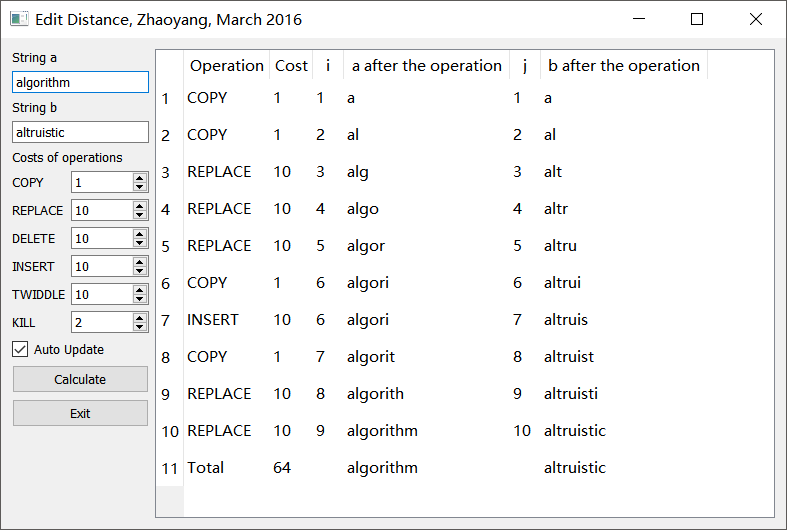
\includegraphics[width=0.75\columnwidth]{screenshot}
}
\problemAnswer{
\subsection{As finding an optimal alignment}
Set of operations
$$\{\mathrm{COPY}, \mathrm{INSERT}, \mathrm{DELETE}, \mathrm{REPLACE}\}$$

Corresponding costs
$$\{-1, 1, 1, 2\}$$

Placing a negative sign before the calculated edit distance gives us the score of optimal alignment.
}

\end{homeworkProblem}


%----------------------------------------------------------------------------------------
%	PROBLEM 2
%----------------------------------------------------------------------------------------


\begin{homeworkProblem}

CRLS Exercises 16.2-6: Solve fractional knapsack problem in $O(n)$ time.

\problemAnswer{
To get $O(n)$ time complexity, we have to avoid sorting. Binary search came into my consideration.

The algorithm can be described as follows:

\begin{quote}
0. Calculate $a_i=\frac{v_i}{w_i}, \forall i$.

1. Find median of $\{a_i\}$, denoted as $m$.

2. Create subsets $$G=\{i: a_i>m\}, E=\{i: a_i=m\}, L=\{i:a_i<m\}$$ Calculate $$W_G=\sum_{i\in G}w_i, W_E=\sum_{i\in E}w_i$$

3. Compare $W_G, W_E$ with $W$.

If $W_G>W$, do recursively on $G$;

If $W_G\leq W$, take every item in $G$, and add $i\in E$ as much as possible. Once we have $W_G+W_G\geq W$, we are done;

Do recursively on $L$ with $W' = W-W_G-W_E$.
\end{quote}

That's where we get pseudo-code, shown below.
}


\problemAnswer{
\begin{codebox}
\Procname{$\proc{Fractional-Knapsack-Problem-Aid(w, v, a, b, W)}$}
\li WG = 0, WE = 0, let G, E, L be new arrays
\li (m, n) = \proc{Find-Median}(a, b);
\li \For i = 1 \To b.length
\li    \Do
            \If a[b[i]] $<$ m
\li                \Then L.add(b[i])
\li         \ElseIf a[b[i]]==m
\li                \Then G.add(b[i]), WG += a[b[i]]
\li         \ElseNoIf E.add(b[i]), WE += a[b[i]]
    \End \End
\li \If WG $>$ W
\li \Then \Return \proc{Fractional-Knapsack-Problem-Aid}(w, v, a, G, W)
    \End
\li let R be a new array
\li S = 0
\li \For i = 1 \To G.length
\li     \Do R.add((G[i], 1)); \End
\li \For i = 1 \To E.length
\li    \Do \If WG + a[E[i]] + S $leq$ W
\li        \Then R.add((E[i], max((W - WG - a[E[i]] - S) / w[a[i]], 1)));
\li    \ElseNoIf \Return R
       \End
    \End
\li \Return R + \proc{Fractional-Knapsack-Problem-Aid}(w, v, a, L, W - WG - WE);
\End
\end{codebox}
\begin{codebox}
\Procname{$\proc{Fractional-Knapsack-Problem(n, w, v, W)}$}

\li let a, b be new arrays
\li \For i = 1 \To n
\li \Do		a[i] = v[i] / w[i], b[i]=[i] \End
\li \Return \proc{Fractional-Knapsack-Problem-Aid}(w, v, a, b, W)
\end{codebox}
}

\problemAnswer{
Let $T(n)$ be running time of problem sized $n$. Then
$$T(n) = T(\frac{n}{2})+\Theta(n)$$

Applying master theorem case 3,
$$T(n) = \Theta(n)$$

QED.
}

\end{homeworkProblem}

%----------------------------------------------------------------------------------------
%	PROBLEM 3
%----------------------------------------------------------------------------------------


\begin{homeworkProblem}

CRLS Problems 16-2 Scheduling to minimize average completion time

a.


\problemAnswer{
The algorithm can be described as follows:

\begin{quote}
0. Sort all the tasks by their processing time increasingly.

1. Process the tasks in that order.
\end{quote}

Proof of correctness:

Suppose we have a optimal scheduling $\{1, 2, 3, ..., n\}$, in which there exists tasks $i$ and $j$ such that $i<j$ and $p_i>p_j$.

$$T=\sum_{k=1}^{n}c_k=\sum_{k=1}^{n}\sum_{m=1}^{k}p_m$$

We may want to swap tasks $i$ and $j$, resulting in another scheduling

$$\{1, 2, ..., i-1, j, i+1, ..., j-1, i, j+1, ..., n\}$$

\begin{equation}
\begin{aligned}
T' & = \sum_{k=1}^{n}c'_k\\
& =
\sum_{k=1}^{i-1}\sum_{m=1}^{k}p_m
+ c'_j
+ \sum_{k=i+1}^{j-1}c'_{k}
+ c'_i
+ \sum_{k=j+1}^{n}\sum_{m=1}^{k}p_m\\
& = \sum_{k=1}^{i-1}\sum_{m=1}^{k}p_m
+   \left( \sum_{k=1}^{i-1}p_k + p_j \right)
+ \sum_{k=i+1}^{j-1}\left(\sum_{q=1}^{i-1}p_q+p_j+\sum_{q=i+1}^{k}p_q\right)
+ \sum_{k=1}^{j}p_k
+ \sum_{k=j+1}^{n}\sum_{m=1}^{k}p_m\\
\end{aligned}
\end{equation}


\begin{equation}
\begin{aligned}
T'-T & =
  \left( \sum_{k=1}^{i-1}p_k + p_j \right)
+ \sum_{k=i+1}^{j-1}\left(\sum_{q=1}^{i-1}p_q+p_j+\sum_{q=i+1}^{k}p_q\right)
+ \sum_{k=1}^{j}p_k
- \sum_{k=i}^{j}\sum_{m=1}^{k}p_m\\
& <
  \sum_{k=1}^{i}p_k
+ \sum_{k=i+1}^{j-1}\sum_{q=1}^{k}p_q
+ \sum_{k=1}^{j}p_k
- \sum_{k=i}^{j}\sum_{m=1}^{k}p_m\\
& =
  \sum_{k=i+1}^{j-1}\sum_{q=1}^{k}p_q
- \sum_{k=i+1}^{j-1}\sum_{m=1}^{k}p_m\\
& =0\\
\end{aligned}
\end{equation}

Now that $T' < T$, it's safe to say that there exists an optimal scheduling $\{1, 2, ..., n\}$ in which $\forall i<j, p_i<p_j$. QED.


Time complexity:

Running time $$T(n)=O(n \log n)$$ where $n$ is number of tasks.
}

b.

\problemAnswer{
We have to decide which task to run at every given time $t$.

\begin{quote}
0. $t=0, T=[]$.

1. $t = t + 1$.

2. Let $A=\{i: r_i\leq t\}$, which represents all the tasks available and unfinished at this moment.

3. If $A=\emptyset$, done. The array $T$ represents the optimal scheduling.

4. Search in $A$ for $i$ minimizing $p_i$. Let $T[t] = i$, meaning that process task $i$ at time $t$.

5. Let $p_i = p_i - 1$, and go back to step 1.

\end{quote}

Proof of correctness:
By contradiction. Swapping tasks, similar to proof of a.


Time complexity:
Running time $T(n)=O(n^2)$, where $n$ is number of tasks.
}

\end{homeworkProblem}


%----------------------------------------------------------------------------------------
%	PROBLEM 4
%----------------------------------------------------------------------------------------


\begin{homeworkProblem}

CRLS Problems 16-5 Off-line caching

a.

\problemAnswer{

\begin{codebox}
\Procname{$\proc{Furthest-In-Future}(r,k)$}
\li let $E$ be new array
\li let $C$ be new array
\li $C[1...k] = r[1...k]$
\li \For $j = k+1$ \To $n$
\li     \Do let $R$ be new array
\li     \For $i = 1$ \To $k$
\li         \Do \If $C[i] = r[j]$
\li         \Then $E[j]=$\const{nil}
            \End
        \End
\li     \For $c = 1$ \To $k$
\li         \Do $E[c]=\infty$
\li         \For $i = j+1$ \To $r$.length
\li             \Do \If $C[c]=r[i]$
\li             \Then $E[i]=$min$(E[i], i)$ \End
           \End
        \End
\li     $m = \infty$
\li     \For $c = 1$ \To $k$
\li         \Do \If $E[c] < m$
\li         \Then $m = E[c]\End$
        \End
\li     E.add(C[m])
    \End
\li \Return E;
\End
\end{codebox}
Running time $T(n)=O(n^2k)$.
}

b. 

\problemAnswer{

}

c.

\problemAnswer{

}

\end{homeworkProblem}



%----------------------------------------------------------------------------------------

\end{document}
